\documentclass{standalone}
\usepackage{tikz}
\usepackage{xcolor-solarized}
\usetikzlibrary{positioning}

\newcommand\commit[2][]{\node[commit, #1] (#2) { \texttt{#2} };}
%\newcommand\commit[2][]{\node[commit, #1] (#2) {};}
\newcommand\commitWork[2][]{\node[commit, fill=solarized-blue!50, #1] (#2) { \texttt{#2} };}
%\newcommand\commitWork[2][]{\node[commit, fill=solarized-blue!50, #1] (#2) {};}
\newcommand\ghost[1]{\coordinate (#1);}
\newcommand\connect[2]{\path[thick] (#1) to[out=0, in=180] (#2);}

\begin{document}
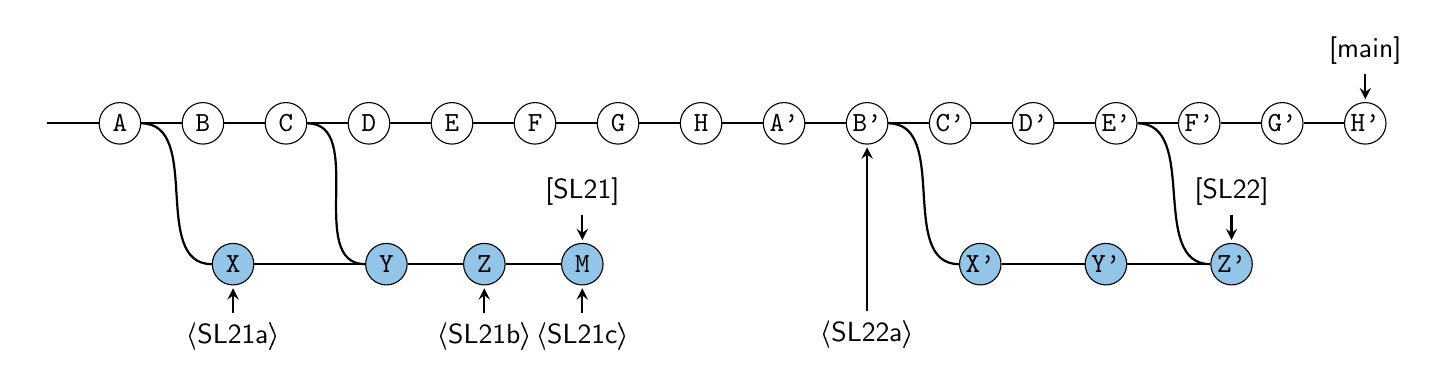
\begin{tikzpicture}

\tikzset{every node}=[font=\sffamily]

\tikzstyle{commit}=[draw, circle, fill=white, inner sep=0.1em, minimum size=1.5em, node distance=3em]
\tikzstyle{every path}=[draw]

\node[] (start) {};
\commit[right of=start]{A};
\commit[right of=A]{B};
\commit[right of=B]{C};
\commit[right of=C]{D};
\commit[right of=D]{E};
\commit[right of=E]{F};
\commit[right of=F]{G};
\commit[right of=G]{H};
%\node[right=4em of H] (end) {};

\connect{start}{A};
\connect{A}{B};
\connect{B}{C};
\connect{C}{D};
\connect{D}{E};
\connect{E}{F};
\connect{F}{G};
\connect{G}{H};
%\connect{H}{end};

\commitWork[below right=4em and 0em of B]{X};
\commitWork[right=4em of X]{Y};
\commitWork[right=2em of Y]{Z};
\commitWork[right=2em of Z]{M};

\connect{A}{X};
\connect{X}{Y};
\connect{Y}{Z};
\connect{Z}{M};
\connect{C}{Y};

\node[below=1em of X] (YW) {\textlangle SL21a\textrangle};
\path[thick, -stealth, shorten >=0.1em] (YW) to[out=north, in=south] (X);

\node[below=1em of Z] (ZW) {\textlangle SL21b\textrangle};
\path[thick, -stealth, shorten >=0.1em] (ZW) to[out=north, in=south] (Z);

\node[below=1em of M] (SL21c) {\textlangle SL21c\textrangle};
\path[thick, -stealth, shorten >=0.1em] (SL21c) to[out=north, in=south] (M);

\node[above=1em of M] (SL21) {[SL21]};
\path[thick, -stealth, shorten >=0.1em] (SL21) to[out=south, in=north] (M);

%\node[above=1em of H] (MAIN) {[main]};
%\path[thick, -stealth, shorten >=0.1em] (MAIN) to[out=south, in=north, outer sep=0.5em] (H);

%\gittag[vA]{vA}{above=of A}{A};

\commit[right of=H]{A'};
\commit[right of=A']{B'};
\commit[right of=B']{C'};
\commit[right of=C']{D'};
\commit[right of=D']{E'};
\commit[right of=E']{F'};
\commit[right of=F']{G'};
\commit[right of=G']{H'};

\connect{H}{A'};
\connect{A'}{B'};
\connect{B'}{C'};
\connect{C'}{D'};
\connect{D'}{E'};
\connect{E'}{F'};
\connect{F'}{G'};
\connect{G'}{H'};

\commitWork[below right=4em and 0em of C']{X'};
\commitWork[right=3em of X']{Y'};
\commitWork[right=3em of Y']{Z'};

\connect{B'}{X'};
\connect{X'}{Y'};
\connect{Y'}{Z'};
\connect{E'}{Z'};

\node[below=6em of B'] (SL22a) {\textlangle SL22a\textrangle};
\path[thick, -stealth, shorten >=0.1em] (SL22a) to[out=north, in=south] (B');

\node[above=1em of Z'] (SL22) {[SL22]};
\path[thick, -stealth, shorten >=0.1em] (SL22) to[out=south, in=north] (Z');

\node[above=1em of H'] (MAIN) {[main]};
\path[thick, -stealth, shorten >=0.1em] (MAIN) to[out=south, in=north, outer sep=0.5em] (H');

\end{tikzpicture}
\end{document}
